The results are reported test by test, then on the committed evidence of the product, and finally against the predictions of \cref{tab:hypotheses}. \Cref{tab:main-results} is the main comparison: for each test, the rule it replaces and the correction, the rejection rate on data without a defect and on data with a planted one, with the Monte Carlo standard error of every rate.

\begin{table}[htbp]
\centering
\small
\caption{The rejection rate of each rule on data without a defect (size, level 0.05) and with a planted defect (power), each with its Monte Carlo standard error, for the three tests: the coverage test at three window ratios, the resilience test with 500 evaluation rows and the situation light with 400 applicants; a rate of 0 or of 1 is printed as its count with the one-sided 95 percent bound $3/R$ of the rule of three, because its sample standard error is zero.}
\label{tab:main-results}
\fitwidth{\begin{tabular}{llccl}
\toprule
Test & Rule & Size (no defect) & Power (planted defect) & Defect \\
\midrule
Coverage & \relax binomial p-value, $m/n = 0.1$ & $0.057 \pm 0.004$ & $0.292 \pm 0.007$ & \relax shape $b=1.10$ \\
Coverage & \relax Beta-Binomial p-value, $m/n = 0.1$ & $0.045 \pm 0.003$ & $0.248 \pm 0.007$ & \relax shape $b=1.10$ \\
Coverage & \relax binomial p-value, $m/n = 1$ & $0.157 \pm 0.006$ & $0.372 \pm 0.008$ & \relax shape $b=1.10$ \\
Coverage & \relax Beta-Binomial p-value, $m/n = 1$ & $0.051 \pm 0.003$ & $0.190 \pm 0.006$ & \relax shape $b=1.10$ \\
Coverage & \relax binomial p-value, $m/n = 4$ & $0.361 \pm 0.008$ & $0.532 \pm 0.008$ & \relax shape $b=1.10$ \\
Coverage & \relax Beta-Binomial p-value, $m/n = 4$ & $0.048 \pm 0.003$ & $0.162 \pm 0.006$ & \relax shape $b=1.10$ \\
Resilience & fixed drop above 0.05 & $0.175 \pm 0.019$ & $0.925 \pm 0.013$ & shift 2 \\
Resilience & fixed drop above 0.10 & $0.048 \pm 0.011$ & $0.703 \pm 0.023$ & shift 2 \\
Resilience & variance z rule & $0.065 \pm 0.012$ & $0.723 \pm 0.022$ & shift 2 \\
Resilience & permutation reference, 199 draws & $0.062 \pm 0.012$ & $0.680 \pm 0.023$ & shift 2 \\
Situation & share cut 0.10 & $0.114 \pm 0.010$ & $400 \text{ of } 400\ (>0.9925)$ & gap 0.4 \\
Situation & share cut 0.20 & $0.014 \pm 0.004$ & $0.968 \pm 0.009$ & gap 0.4 \\
\bottomrule
\end{tabular}}
\end{table}


\subsection{The coverage test}

\paragraph{Size.} At a test window a tenth of the calibration window the binomial test is close to its level, with \CovSinBinA{} (standard error \CovSeBinA{}) at $(n,m)=(20000,2000)$, and the Beta-Binomial test is at \CovSinBBA{} (\CovSeBBA{}). The two diverge as the window grows. At equal windows, $(n,m)=(2000,2000)$, the binomial test rejects an exchangeable window in \CovSinBinB{} of the replications (\CovSeBinB{}) and the Beta-Binomial test in \CovSinBBB{} (\CovSeBBB{}); at a test window four times the calibration window, $(1000,4000)$, the binomial test rejects in \CovSinBinC{} (\CovSeBinC{}) and the Beta-Binomial test in \CovSinBBC{} (\CovSeBBC{}). The exact sizes, summed over the rejection regions, are \CovExBinB{} and \CovExBBB{} at equal windows and \CovExBinC{} and \CovExBBC{} at four times; the simulated and exact sizes agree to within the Monte Carlo error. Over the \CovGridCells{} window pairs of the grid (three calibration sizes and seven window ratios) the simulated size of the binomial test lies in \CovSimBinMinOne{} to \CovSimBinMaxOne{} at equal windows and in \CovSimBinMinFour{} to \CovSimBinMaxFour{} at four times the calibration window, and the Beta-Binomial test never exceeds \CovBBMaxRate{}; \CovBBOverBound{} cells have a rate above $0.05$ plus two standard errors, and its exact size never exceeds \CovBBMaxExact{}. Among the \CovMcCompare{} comparisons of a simulated size with the exact size of the same rule, the largest difference is \CovMcExactMaxZ{} standard errors. The engine's function and the vectorised tables used for the variants disagree on \CovEngineMismatches{} replications of \CovTotalReps{}.

\Cref{tab:exact-size} gives every cell, and \cref{fig:coverage-size} shows the exact size and the normal approximation of \cref{prop:binomial-size} as curves and the simulated rates as points with two-standard-error bars. The simulated points of the three calibration sizes fall on the one curve of the ratio $m/n$ on the logarithmic axis, which says that the size of the binomial test is a function of the ratio and, for the sizes of this grid, almost not of $n$ alone; the Beta-Binomial points lie on the line of the level, below it at the smallest windows where the discreteness of the law makes the test conservative (exact sizes \CovExBBMinTenth{} to \CovExBBMaxTenth{} at a tenth of the calibration window).

\begin{table}[htbp]
\centering
\small
\caption{The size of the binomial and of the Beta-Binomial coverage test at level 0.05 for calibration windows of 200, 1,000 and 5,000 rows and test windows from 0.1 to 8 times as long (every cell of the size grid): the exact sum of the Beta-Binomial law, the normal approximation of the binomial size, and the engine's functions on 4,000 seeded replications with the standard error.}
\label{tab:exact-size}
\fitwidth{\begin{tabular}{rrrccccc}
\toprule
$n$ & $m$ & $m/n$ & Binomial, exact & Binomial, normal & Binomial, simulated & Beta-Binomial, exact & Beta-Binomial, simulated \\
\midrule
200 & 20 & 0.1 & 0.0504 & 0.0610 & $0.048 \pm 0.003$ & 0.0152 & $0.015 \pm 0.002$ \\
200 & 50 & 0.25 & 0.0484 & 0.0787 & $0.054 \pm 0.004$ & 0.0484 & $0.054 \pm 0.004$ \\
200 & 100 & 0.5 & 0.0992 & 0.1084 & $0.106 \pm 0.005$ & 0.0366 & $0.038 \pm 0.003$ \\
200 & 200 & 1 & 0.1496 & 0.1642 & $0.148 \pm 0.006$ & 0.0410 & $0.037 \pm 0.003$ \\
200 & 400 & 2 & 0.2466 & 0.2558 & $0.244 \pm 0.007$ & 0.0497 & $0.048 \pm 0.003$ \\
200 & 800 & 4 & 0.3699 & 0.3786 & $0.375 \pm 0.008$ & 0.0499 & $0.053 \pm 0.004$ \\
200 & 1,600 & 8 & 0.5055 & 0.5116 & $0.496 \pm 0.008$ & 0.0491 & $0.050 \pm 0.003$ \\
1,000 & 100 & 0.1 & 0.0550 & 0.0615 & $0.054 \pm 0.004$ & 0.0362 & $0.035 \pm 0.003$ \\
1,000 & 250 & 0.25 & 0.0712 & 0.0794 & $0.072 \pm 0.004$ & 0.0462 & $0.046 \pm 0.003$ \\
1,000 & 500 & 0.5 & 0.0987 & 0.1093 & $0.103 \pm 0.005$ & 0.0436 & $0.041 \pm 0.003$ \\
1,000 & 1,000 & 1 & 0.1562 & 0.1655 & $0.162 \pm 0.006$ & 0.0473 & $0.046 \pm 0.003$ \\
1,000 & 2,000 & 2 & 0.2532 & 0.2574 & $0.263 \pm 0.007$ & 0.0494 & $0.046 \pm 0.003$ \\
1,000 & 4,000 & 4 & 0.3763 & 0.3803 & $0.361 \pm 0.008$ & 0.0496 & $0.048 \pm 0.003$ \\
1,000 & 8,000 & 8 & 0.5104 & 0.5132 & $0.512 \pm 0.008$ & 0.0495 & $0.053 \pm 0.004$ \\
5,000 & 500 & 0.1 & 0.0543 & 0.0616 & $0.058 \pm 0.004$ & 0.0462 & $0.051 \pm 0.003$ \\
5,000 & 1,250 & 0.25 & 0.0764 & 0.0796 & $0.077 \pm 0.004$ & 0.0472 & $0.046 \pm 0.003$ \\
5,000 & 2,500 & 0.5 & 0.1080 & 0.1095 & $0.108 \pm 0.005$ & 0.0498 & $0.046 \pm 0.003$ \\
5,000 & 5,000 & 1 & 0.1614 & 0.1657 & $0.161 \pm 0.006$ & 0.0490 & $0.045 \pm 0.003$ \\
5,000 & 10,000 & 2 & 0.2561 & 0.2577 & $0.258 \pm 0.007$ & 0.0495 & $0.048 \pm 0.003$ \\
5,000 & 20,000 & 4 & 0.3787 & 0.3807 & $0.378 \pm 0.008$ & 0.0497 & $0.047 \pm 0.003$ \\
5,000 & 40,000 & 8 & 0.5121 & 0.5135 & $0.513 \pm 0.008$ & 0.0497 & $0.046 \pm 0.003$ \\
\bottomrule
\end{tabular}}
\end{table}


\begin{figure}[htbp]
\centering
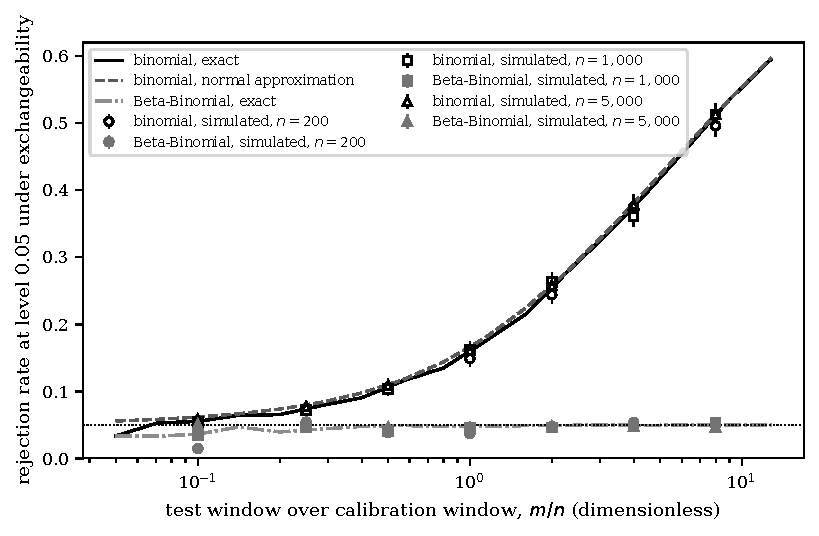
\includegraphics[width=0.92\textwidth]{coverage_size}
\caption{Rejection rate of the binomial and of the Beta-Binomial coverage test at the level 0.05 on exchangeable data, against the ratio of the test window to the calibration window; curves are the exact size and the normal approximation of the binomial test for 1,000 calibration rows, and points are the simulated rates for 200, 1,000 and 5,000 rows with two-standard-error bars over 4,000 replications.}
\label{fig:coverage-size}
\end{figure}

\paragraph{The rejection regions.} The size excess has a direct reading in terms of the coverage. At $n=m=1000$ the binomial test accepts an empirical coverage between \RegionBinLo{} and \RegionBinHi{}, and the Beta-Binomial test between \RegionBBLo{} and \RegionBBHi{}: the exact law of the count is wider than the binomial law, and the corrected test accepts a band of coverages that the binomial test would call a failure. \Cref{fig:rejection-regions} draws the two p-values as functions of the coverage, with the level 0.05 as a horizontal line; the binomial p-value falls below the level on the shoulders of the Beta-Binomial one.

\begin{figure}[htbp]
\centering
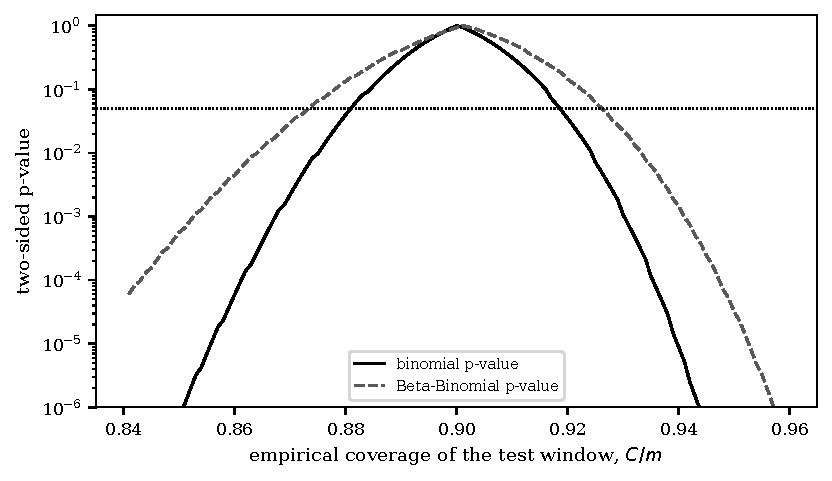
\includegraphics[width=0.92\textwidth]{rejection_regions}
\caption{The binomial and the Beta-Binomial two-sided p-value of a covered count as a function of the empirical coverage of a test window of 1,000 rows against a calibration window of 1,000 rows and the target 0.90, on a logarithmic axis, with the level 0.05 as the dotted line; the Beta-Binomial p-value stays above the level over a wider range of coverages.}
\label{fig:rejection-regions}
\end{figure}

\paragraph{Power.} With a drift of the test scores of shape $b=1.10$ the binomial test rejects in \CovPowBinBTen{} of the replications at equal windows and \CovPowBinCTen{} at four times the calibration window, against \CovPowBBBTen{} and \CovPowBBCTen{} for the Beta-Binomial test. The correction looks like a loss of power by that comparison, and \cref{fig:coverage-power} shows why the comparison is not meaningful: when the power is plotted against the coverage lost, the binomial test starts at its size excess (\CovSinBinB{} and \CovSinBinC{} at no loss) and rises on a curve that lies above the Beta-Binomial one by about the size excess, and the binomial test with the cut calibrated to the exact size 0.05 lies on the Beta-Binomial curve. At $b=1.10$ the calibrated binomial test rejects in \CovPowOracleBTen{} and \CovPowOracleCTen{} of the replications at the two windows, within \ExPowGapMax{} (exact) of the Beta-Binomial test over every window pair and drift shape of the exact power curves, as \cref{conj:power} states. The power that the binomial test appears to have in excess of the Beta-Binomial test is its size.

\begin{figure}[htbp]
\centering
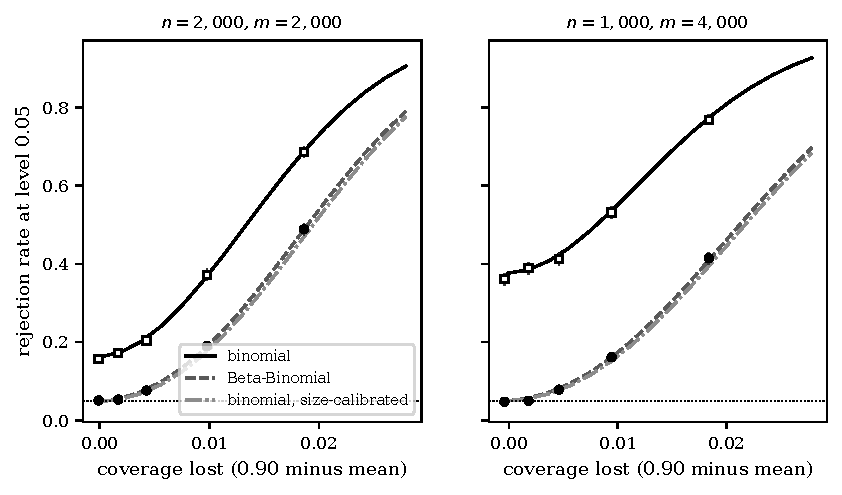
\includegraphics[width=\textwidth]{coverage_power}
\caption{Power of the binomial, the Beta-Binomial and the size-calibrated binomial coverage test against the coverage lost to the planted drift (0.90 minus the mean coverage), for equal windows of 2,000 rows (left) and for 1,000 calibration rows and 4,000 test rows (right); curves are exact, and points with two-standard-error bars are simulated over 4,000 replications.}
\label{fig:coverage-power}
\end{figure}

\subsection{The committed coverage evidence}

\Cref{tab:committed-conformal} lists the five conformal coverage rows of the committed shift variant of the credit model, with both p-values the engine returns, and \cref{fig:committed-p} draws the two p-values side by side on a logarithmic scale. The calibration window holds \CmNcal{} rows and each test window \CmBaseM{} rows (\CmPoolM{} for the pooled window), so the ratio $m/n$ is about 2.1, a ratio at which the binomial test has a size of about 0.25 (\cref{tab:exact-size}). At the baseline window, whose coverage is \CmBaseCov{}, both tests accept (p-values \CmBaseBB{} and \CmBaseBin{}) and the light is \CmBaseLight{}. At the windows shifted by 0.25 and by 0.5 times the size of the Federal Reserve higher-risk shift the coverage falls to \CmQuarterCov{} and \CmHalfCov{} and both p-values are far below $0.01$ (\CmQuarterBB{} and \CmHalfBB{} for the Beta-Binomial test), so the lights are \CmQuarterLight{} and \CmHalfLight{} whichever p-value is read; the pooled window is also \CmPoolLight{} (\CmPoolBB{}). The coverage is not monotone in the multiple of the shift (\CmQuarterCov{}, \CmHalfCov{} and then \CmOneCov{}); the three windows are the same holdout displaced by 0.25, 0.5 and 1 times one displacement of the leading features, and the committed document of the case reports the three values without a mechanism for the rise, which is not tested here. The window shifted by the full size has the coverage \CmOneCov{}, which is below the target by 0.02: the Beta-Binomial p-value is \CmOneBB{}, so the light is \CmOneLight{}, whereas the binomial p-value of the same count is \CmOneBin{}, below the red level 0.01, and a rule that read the binomial p-value would have set the light to red. This is the one window of five whose light the correction changes, and it changes it in the direction the size calculation predicts: after a calibration on \CmNcal{} rows, a coverage of \CmOneCov{} on \CmOneM{} rows is a count that the exact law of exchangeable data produces with a probability of \CmOneBB{} (the p-value), and that the binomial law, which ignores the randomness of the calibration quantile, calls \CmOneBin{} likely. Recomputing every committed p-value from its covered count with the engine function reproduces the committed value to \CmRecomputeDiff{} in the base-10 logarithm.

\begin{table}[htbp]
\centering
\small
\caption{The conformal coverage rows of the committed shift variant of the gradient-boosting model fitted on the Polish company bankruptcy data, evaluated on the locked holdout shifted by sizes taken from the Federal Reserve corporate portfolios: the calibration and test sizes, the empirical coverage against the target 0.90, both p-values of the engine and the light the Beta-Binomial p-value sets; the light never reads the binomial one.}
\label{tab:committed-conformal}
\fitwidth{\begin{tabular}{lrrcccl}
\toprule
Window & $n$ & $m$ & Coverage & $p$ Beta-Binomial & $p$ binomial & Light \\
\midrule
baseline & 1,471 & 3,151 & 0.8946 & 0.523 & 0.313 & green \\
higher risk x0.25 & 1,471 & 3,151 & 0.7509 & 2.13e-35 & 3.69e-127 & red \\
higher risk x0.5 & 1,471 & 3,151 & 0.7099 & 4.56e-52 & 1.19e-194 & red \\
higher risk x1 & 1,471 & 3,151 & 0.8800 & 0.0372 & 0.000258 & amber \\
pooled & 1,471 & 12,604 & 0.8089 & 2.86e-20 & 2.16e-207 & red \\
\bottomrule
\end{tabular}}
\end{table}


\begin{figure}[htbp]
\centering
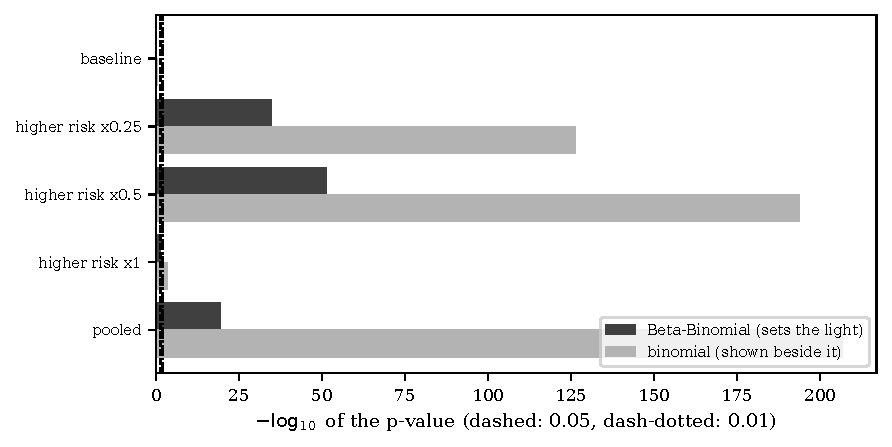
\includegraphics[width=0.92\textwidth]{committed_p}
\caption{Minus the base-10 logarithm of the Beta-Binomial and of the binomial p-value of each committed conformal coverage window of the credit-model shift case, with the levels 0.05 (dashed) and 0.01 (dash-dotted); bars longer than 8 are cut at 8, with their value printed. The two p-values set the same light on four windows; on the shifted and pooled windows both are far below 0.01 and differ by many orders of magnitude, and on the window of full Federal Reserve shift the binomial p-value (\CmOneBin{}) falls below 0.01 while the Beta-Binomial one (\CmOneBB{}) does not.}
\label{fig:committed-p}
\end{figure}

\subsection{The resilience test}

\paragraph{The null drop.} Without shift the AUC drop on the worst quarter is not centred on zero. At 500 evaluation rows its mean is \ShMeanDropCZ{}, its standard deviation \ShSdDropCZ{} and its 95th percentile \ShQNinetyFiveCZ{}, so a fixed cut of 0.05 is exceeded by \ShRateFixedFiveCZ{} of the null drops and a cut of 0.10 by \ShRateFixedTenCZ{}. \Cref{fig:shift-drops} shows the two histograms of the drops at shift 0 and shift 2. The mean of the drops that the permutation reference draws is \ShNullMeanCZ{}, close to the mean \ShMeanDropCZ{} of the observed null drops, which is what an exchangeable reference should give; the p-value reads the observed drop against the upper tail of the reference, and the rates below put its upper tail within about two standard errors of the exact grid size.

\begin{figure}[htbp]
\centering
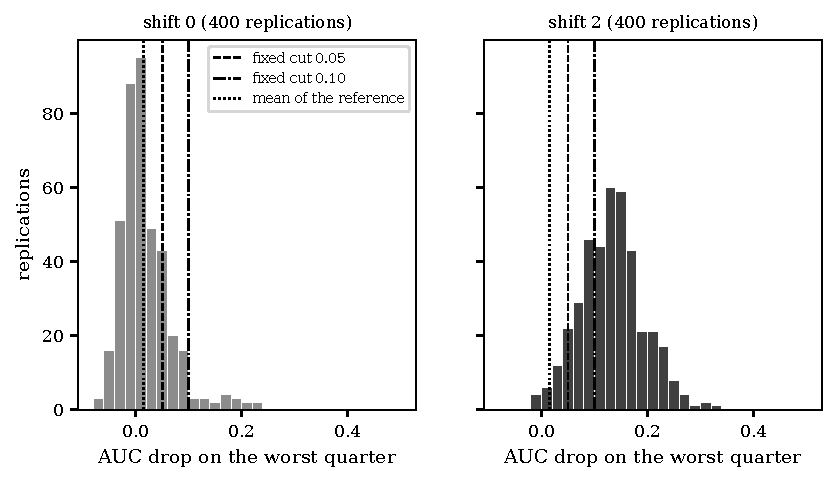
\includegraphics[width=\textwidth]{shift_drops}
\caption{Histograms of the AUC drop on the worst quarter of 500 evaluation rows over 400 replications without shift (left) and with a planted shift of two standard deviations (right), with the fixed cuts 0.05 and 0.10 and the mean of the null drops of the permutation reference as vertical lines.}
\label{fig:shift-drops}
\end{figure}

\paragraph{Size and power at 500 rows.} The fixed cut 0.05 raises a false alarm in \ShRateFixedFiveCZ{} of the shift-free replications (standard error \ShSeFixedFiveCZ{}) and the fixed cut 0.10 in \ShRateFixedTenCZ{} (\ShSeFixedTenCZ{}); the z rule gives \ShRateZruleCZ{} (\ShSeZruleCZ{}) and the permutation reference with 199 draws \ShRatePermCZ{} (\ShSePermCZ{}). At the planted shift of two standard deviations the four rules reject in \ShRateFixedFiveCT{}, \ShRateFixedTenCT{}, \ShRateZruleCT{} and \ShRatePermCT{} of the replications. The permutation reference therefore detects a planted shift less often than the fixed cut 0.05 in every cell with a shift, by at least \ShPermPowerGapMin{}, and the larger part of the difference is the false alarms of the cut. A fixed cut set at the 95th percentile of the null drops of the same cell, \ShOracleCut{} at 500 rows, has by construction the size \ShOracleRateZ{} and the power \ShOracleRateT{} at shift 2. Of the difference \ShFixedPermDiffT{} in power between the fixed cut 0.05 and the reference at shift 2, the calibrated cut also gives up \ShFixedOracleDiffT{}, and the reference gives up a further \ShOracleDiffT{}, at a standard error of \ShOracleDiffSe{}; the calibrated cut needs a simulation of the null that a validation team does not have.

\paragraph{The size of a fixed cut depends on the evaluation sample.} \Cref{tab:shift-eval-size} and \cref{fig:shift-eval-size} give the four rules at the four evaluation sizes. The fixed cut 0.05 raises a false alarm in \ShRateFixedFiveAZ{}, \ShRateFixedFiveBZ{}, \ShRateFixedFiveCZ{} and \ShRateFixedFiveDZ{} of the replications at 125, 250, 500 and 1,000 rows, and the cut 0.10 in \ShRateFixedTenAZ{}, \ShRateFixedTenBZ{}, \ShRateFixedTenCZ{} and \ShRateFixedTenDZ{}: the size falls as the evaluation sample grows, because the spread of the null drop falls, and the cut that would have size 0.05 (the 95th percentile of the null drops) is \ShQNinetyFiveAZ{}, \ShQNinetyFiveBZ{}, \ShQNinetyFiveCZ{} and \ShQNinetyFiveDZ{}. The cut 0.10 is close to calibrated at 500 rows and oversized at 125 rows, and a team that tuned it at 500 rows would carry a size of \ShRateFixedTenAZ{} to the smaller design. The permutation reference with 199 draws stays between \ShRatePermAZ{} and \ShRatePermCZ{} at every size, and the z rule between \ShRateZruleBZ{} and \ShRateZruleCZ{}.

The power of the permutation reference at shift 2 is \ShRatePermAT{}, \ShRatePermBT{}, \ShRatePermCT{} and \ShRatePermDT{} over the four sizes and the power of the fixed cut 0.05 is \ShRateFixedFiveAT{}, \ShRateFixedFiveBT{}, \ShRateFixedFiveCT{} and \ShRateFixedFiveDT{}; the difference is \ShPowGapAT{}, \ShPowGapBT{}, \ShPowGapCT{} and \ShPowGapDT{}, so it narrows as the evaluation sample grows. The z rule has less power than the reference at 125 and 250 rows (\ShRateZruleAT{} and \ShRateZruleBT{} against \ShRatePermAT{} and \ShRatePermBT{}) and more at 500 and 1,000 rows (\ShRateZruleCT{} and \ShRateZruleDT{} against \ShRatePermCT{} and \ShRatePermDT{}).

\begin{table}[htbp]
\centering
\small
\caption{The size (shift 0) and the power (shift 2) of four rules of the resilience test as the evaluation sample grows from 125 to 1,000 rows, with the development sample twice as large; rates with their standard errors over the replications of each cell.}
\label{tab:shift-eval-size}
\fitwidth{\begin{tabular}{llcccc}
\toprule
Rule & Rate & $n_{\mathrm{eval}}=125$ & 250 & 500 & 1,000 \\
\midrule
fixed 0.05 & size & $0.254 \pm 0.022$ & $0.212 \pm 0.020$ & $0.175 \pm 0.019$ & $0.125 \pm 0.017$ \\
fixed 0.05 & power & $0.709 \pm 0.023$ & $0.853 \pm 0.018$ & $0.925 \pm 0.013$ & $0.993 \pm 0.004$ \\
fixed 0.10 & size & $0.098 \pm 0.015$ & $0.068 \pm 0.013$ & $0.048 \pm 0.011$ & $0.040 \pm 0.010$ \\
fixed 0.10 & power & $0.520 \pm 0.025$ & $0.635 \pm 0.024$ & $0.703 \pm 0.023$ & $0.792 \pm 0.020$ \\
z rule & size & $0.035 \pm 0.009$ & $0.030 \pm 0.009$ & $0.065 \pm 0.012$ & $0.045 \pm 0.010$ \\
z rule & power & $0.188 \pm 0.020$ & $0.422 \pm 0.025$ & $0.723 \pm 0.022$ & $0.940 \pm 0.012$ \\
permutation, 199 & size & $0.048 \pm 0.011$ & $0.055 \pm 0.011$ & $0.062 \pm 0.012$ & $0.052 \pm 0.011$ \\
permutation, 199 & power & $0.317 \pm 0.023$ & $0.527 \pm 0.025$ & $0.680 \pm 0.023$ & $0.870 \pm 0.017$ \\
\bottomrule
\end{tabular}}
\end{table}


\begin{figure}[htbp]
\centering
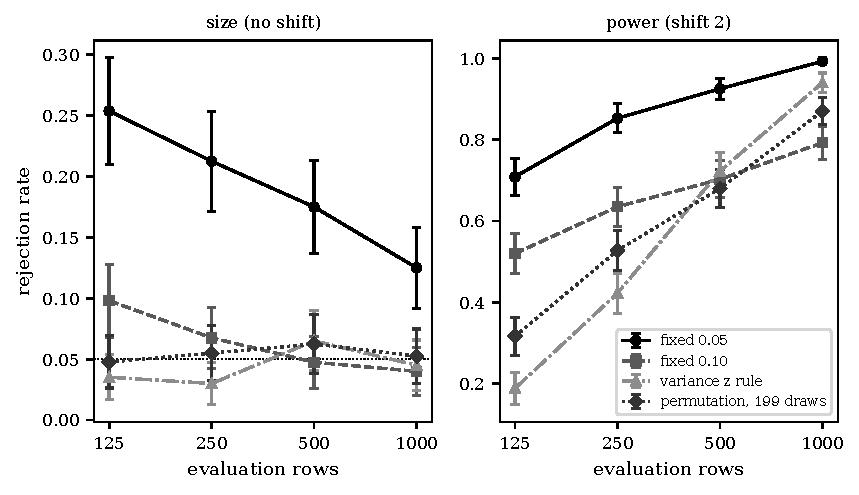
\includegraphics[width=\textwidth]{shift_eval_size}
\caption{Size at shift 0 (left) and power at a planted shift of two standard deviations (right) of four rules of the resilience test, the fixed cuts 0.05 and 0.10, the variance z rule and the permutation reference with 199 draws, against the number of evaluation rows, with two-standard-error bars over 400 replications per cell.}
\label{fig:shift-eval-size}
\end{figure}

\paragraph{The number of draws.} The permutation reference with 19 draws never rejects: the smallest attainable p-value is \GranSmallestNineteen{}, which is not below $0.05$, and the measured rate is \ShRatePermNineteenCZ{} at every size and shift. With 39, 99 and 199 draws the pooled sizes over the four evaluation sizes are \ShPermPooledThirtyNine{}, \ShPermPooledNinetyNine{} and \ShPermPooledFull{}, with standard errors of about \ShPermPooledSeFull{}, against the exact sizes \GranExactThirtyNine{}, \GranExactNinetyNine{} and \GranExactFull{} that \cref{prop:permutation} gives for an exchangeable reference; the measured sizes lie above the exact ones by \ShPermExcessThirtyNine{}, \ShPermExcessNinetyNine{} and \ShPermExcessFull{}, which is \ShPermExcessZMin{} to \ShPermExcessZMax{} of the measured standard errors and \ShPermExcessZExactMin{} to \ShPermExcessZExactMax{} of the standard error of the exact null rate. The three readings are not three observations: the references with 39 and 99 draws are the first draws of the 199 of the same replications, so they share replications and draws, and the common sign is one observation. At 500 rows the size is \ShRatePermCZ{} (\ShSePermCZ{}), within the bound of 0.05 plus two standard errors but above the exact 0.045 that an exchangeable reference gives. A possible cause, not tested here, is the approximate exchangeability of the engine's construction (a pseudo-development set of $n_d-n_e$ rows); no experiment varies the size of that set. The power rises with the number of draws, from \ShRatePermThirtyNineCT{} with 39 to \ShRatePermNinetyNineCT{} with 99 and \ShRatePermCT{} with 199 at 500 rows and shift 2 (\cref{fig:shift-draws}). The red light of the engine needs a p-value below $0.01$, which a reference with fewer than \RedMinDraws{} draws cannot give.

\begin{figure}[htbp]
\centering
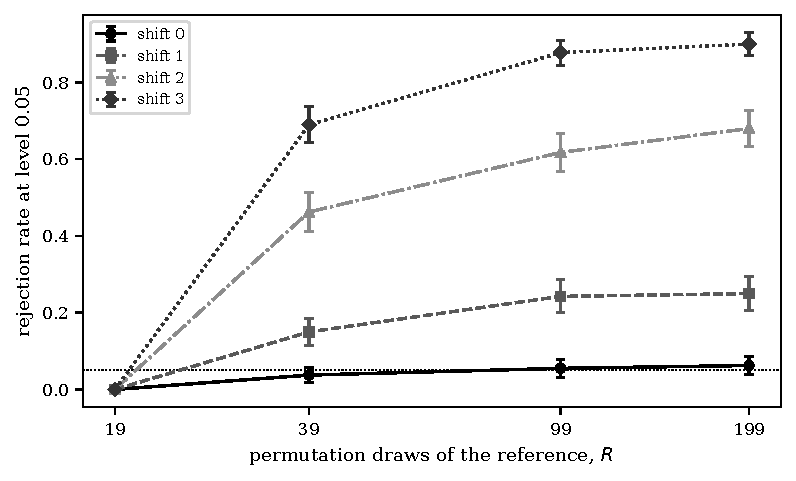
\includegraphics[width=0.85\textwidth]{shift_draws}
\caption{Rejection rate of the permutation reference at the level 0.05 as a function of its number of draws, at 500 evaluation rows and planted shifts of 0, 1, 2 and 3 standard deviations, with two-standard-error bars over 400 replications; the dotted line is the level 0.05.}
\label{fig:shift-draws}
\end{figure}

\paragraph{The committed resilience row.} The committed resilience row of the credit-model shift case has \CmResN{} evaluation rows, a worst share of 0.10 and the observed drop \CmResDrop{}. The \CmResDraws{} draws of the reference have a mean of \CmResNullMean{} and a 95th percentile of \CmResNullP{}, and none of them reaches the observed drop, so the p-value is the smallest the reference can give, \CmResP{}, and the light is red. A fixed cut of 0.05 would also have fired; the reference differs in that it says how far the drop is from what a shift-free sample of the same size gives.

\subsection{The situation-testing light}

\paragraph{The null law of the share.} With 400 applicants on the threshold-bias plant the protected group has about \SiComplainantsSmallZ{} complainants, the share of significant complainants has a mean of \SiMeanShareSmallZ{} and a standard deviation of \SiSdShareSmallZ{} without bias, and the design effect of \cref{eq:design-effect} is \SiDesignSmallZ{}; with 1,000 applicants the complainants number \SiComplainantsLargeZ{}, the mean share is \SiMeanShareLargeZ{}, the standard deviation \SiSdShareLargeZ{} and the design effect \SiDesignLargeZ{}. Independent complainants at the level 0.05 would give a standard deviation of \SiIndepSd{} at 200 complainants. \Cref{fig:situation-null-share} shows the two null histograms with the cuts 0.10 and 0.20: the distribution is right-skewed, with a tail that reaches above 0.10 at 400 applicants and almost not at 1,000.

\begin{figure}[htbp]
\centering
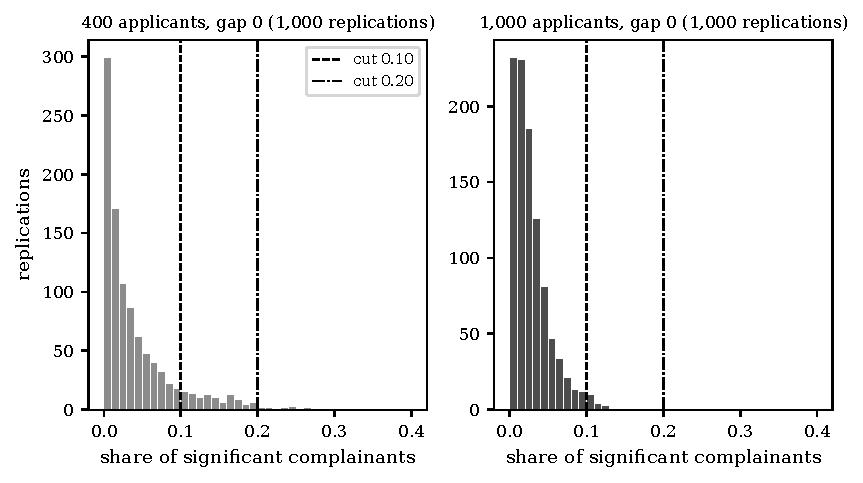
\includegraphics[width=\textwidth]{situation_null_share}
\caption{Histograms of the share of significant complainants without bias for 400 applicants over 1,000 replications (left) and 1,000 applicants over 1,000 replications (right), on the threshold-bias plant, with the amber cuts 0.10 and 0.20 as vertical lines; the right tail beyond 0.10 shrinks sharply as the number of applicants grows.}
\label{fig:situation-null-share}
\end{figure}

\paragraph{Size and power of the cuts.} With 400 applicants the cut 0.10 fires in \SiRateCutTenSmallZ{} of the null replications (standard error \SiSeCutTenSmallZ{}) and the cut 0.20 in \SiRateCutTwentySmallZ{} (\SiSeCutTwentySmallZ{}). At the planted gap 0.4 they detect the bias in \SiRateCutTenSmallC{} and \SiRateCutTwentySmallC{} of the replications and at the gap 0.8 in every replication. At the small gaps the cut 0.20 has less power: \SiRateCutTwentySmallB{} against \SiRateCutTenSmallB{} at the gap 0.2, and \SiRateCutTwentySmallA{} against \SiRateCutTenSmallA{} at the gap 0.1 (\cref{tab:situation-ablation}). With 1,000 applicants the cut 0.10 fires in \SiRateCutTenLargeZ{} of the null replications and the cut 0.20 in \SiRateCutTwentyLargeZ{}; the cut 0.20 detects the gap 0.2 in \SiRateCutTwentyLargeB{} of the replications. \Cref{fig:situation-cuts} shows the rates of the seven cuts at each gap: the curves of the null and of the planted gaps cross, so that every cut is a choice of a point on a trade between size and power that depends on the number of applicants.

\begin{figure}[htbp]
\centering
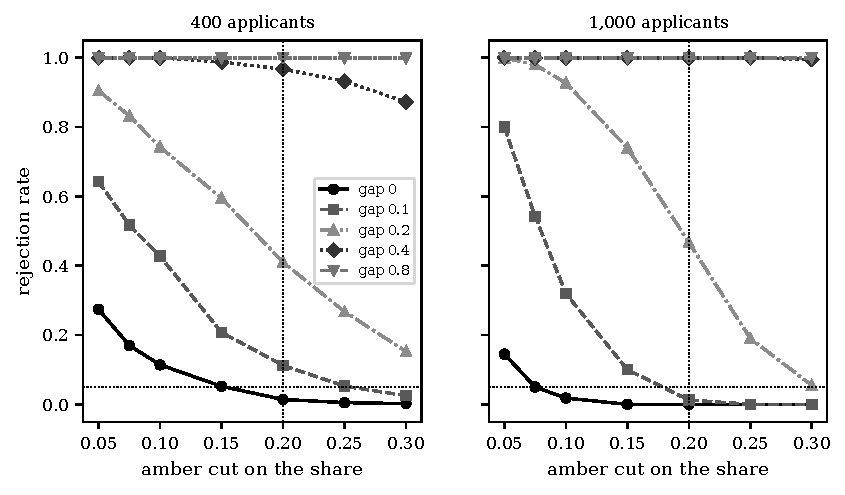
\includegraphics[width=\textwidth]{situation_cuts}
\caption{Rejection rate of the share cut as a function of the cut for 400 applicants (left) and 1,000 applicants (right) and the planted gaps 0, 0.1, 0.2, 0.4 and 0.8, over 1,000 replications at gap 0 and 400 at the others; the vertical dotted line is the engine's cut 0.20 and the horizontal dotted line the level 0.05.}
\label{fig:situation-cuts}
\end{figure}

\paragraph{A second data-generating process.} On the design of the engine's own size-and-power suite, with attributes that are independent of the decision, the null law of the share is different (\cref{tab:situation-designs}). At 400 applicants the cut 0.10 fires in \SiInRateCutTenSmallZ{} of the null replications (\SiInSeCutTenSmallZ{}) and the cut 0.20 in \SiInRateCutTwentySmallZ{} (\SiInSeCutTwentySmallZ{}), against \SiRateCutTenSmallZ{} and \SiRateCutTwentySmallZ{} on the threshold-bias plant. The engine's suite records a size of \EngSiSizeTwenty{} (standard error \EngSiSeTwenty{}) for the cut 0.20 and \EngSiSizeTen{} for the former cut 0.10 at 400 applicants and 30 neighbours on that design, and the values measured here, \SiInRateCutTwentySmallZ{} and \SiInRateCutTenSmallZ{}, reproduce them. At 1,000 applicants the sizes on the second design are \SiInRateCutTenLargeZ{} and \SiInRateCutTwentyLargeZ{}. The two designs differ in the size of the same cut by a factor of about two at 400 applicants, and the size of a cut at one number of applicants does not carry to another on either design. The cut chosen by \cref{eq:cut-rule} on the grid of the experiments is therefore \SiChosenThrSmall{} on the threshold-bias plant at 400 applicants (size \SiRateCutFifteenSmallZ{}, standard error \SiSeCutFifteenSmallZ{}) and \SiChosenIndSmall{} on the second design, where the cut 0.15 has size \SiInRateCutFifteenSmallZ{}.

\begin{table}[htbp]
\centering
\small
\caption{The null law of the share of significant complainants and the size of the amber cuts 0.10 and 0.20 on two planted designs without bias, for 400 and for 1,000 applicants: the mean number of complainants, the mean and standard deviation of the share, the variance of the count over the binomial variance, and the size with its Monte Carlo standard error over 1,000 and 2,000 replications.}
\label{tab:situation-designs}
\fitwidth{\begin{tabular}{llrrrrcc}
\toprule
Design & Applicants & Complainants & Mean share & SD of share & Design effect & Size, cut 0.10 & Size, cut 0.20 \\
\midrule
threshold-bias plant & 400 & 200 & 0.041 & 0.050 & 10.6 & $0.114 \pm 0.010$ & $0.014 \pm 0.004$ \\
threshold-bias plant & 1,000 & 500 & 0.028 & 0.023 & 5.8 & $0.018 \pm 0.004$ & $0 \text{ of } 1{,}000\ (<0.0030)$ \\
independent attributes & 400 & 160 & 0.055 & 0.062 & 12.8 & $0.195 \pm 0.009$ & $0.035 \pm 0.004$ \\
independent attributes & 1,000 & 400 & 0.055 & 0.038 & 12.3 & $0.128 \pm 0.007$ & $0.0005 \pm 0.0005$ \\
\bottomrule
\end{tabular}}
\end{table}


\paragraph{The other rules.} The one-sided binomial test of the count, which treats the complainants as independent, has size \SiRateCountBinSmallZ{} at 400 applicants on the threshold-bias plant and \SiInRateCountBinSmallZ{} on the second design, three to five times the level; the rule that rejects when one complainant is significant at the Bonferroni level has size \SiRateBonfSmallZ{} and \SiInRateBonfSmallZ{} and detects the gap 0.2 in \SiRateBonfSmallB{} of the replications, close to the share cut 0.20 (\SiRateCutTwentySmallB{}, within the error) and less than the share cut 0.10 (\SiRateCutTenSmallB{}).

\subsection{The committed fairness evidence}

\Cref{tab:committed-fair} lists the situation-testing row of each of the six committed year pairs of the mortgage decisions of Delaware. The number of complainants is between \CmFairQMin{} and \CmFairQMax{}, an order of magnitude or more above the \SiComplainantsSmallZ{} and \SiComplainantsLargeZ{} of the plants, and the shares of significant complainants are between \CmFairMin{} and \CmFairMax{}. With the amber cut 0.20, \CmFairAmber{} pairs are amber and \CmFairGreen{} are green; with the former cut 0.10 all \CmFairAboveTen{} pairs, whose share exceeds it, would be amber. The two green pairs have shares of \CmFairGreenLo{} and \CmFairGreenHi{}, just below the cut. The cut 0.20 was measured at 400 applicants, and the null share narrows as the complainants become more numerous (\cref{tab:situation-designs}), so at the committed size a null share at 0.20 is rarer than the measured size suggests; how much rarer is not measured here. The size of neither cut is measured at the committed number of complainants, so the two green pairs are not shown to be a gain: the null mean share of the plants is at most \SiNullMeanMax{}, and the green pairs have shares at least \CmFairGreenOverNull{} times that value. The cut 0.10 has the higher power at small gaps (\cref{tab:situation-ablation}), and at 1,000 applicants on the threshold-bias plant its size is \SiRateCutTenLargeZ{}, below the level, so setting the two pairs green may cost sensitivity and is not shown to improve the light.

\begin{table}[htbp]
\centering
\small
\caption{The situation-testing row of each committed Delaware mortgage year pair: the complainants of the protected group, how many are significant at level 0.05 with thirty neighbours, their share, the amber cut point the engine applies and the light that follows; the light is never red.}
\label{tab:committed-fair}
\fitwidth{\begin{tabular}{lrrccl}
\toprule
Year pair & Complainants & Significant & Share & Amber cut & Light \\
\midrule
2018-19 & 4,485 & 1,179 & 0.2629 & 0.20 & amber \\
2019-20 & 4,655 & 1,123 & 0.2412 & 0.20 & amber \\
2020-21 & 5,644 & 1,056 & 0.1871 & 0.20 & green \\
2021-22 & 8,113 & 1,616 & 0.1992 & 0.20 & green \\
2022-23 & 6,421 & 1,442 & 0.2246 & 0.20 & amber \\
2023-24 & 4,919 & 1,199 & 0.2437 & 0.20 & amber \\
\bottomrule
\end{tabular}}
\end{table}


\subsection{The predictions}

\Cref{tab:hypotheses} gives the outcome of each prediction. \HypHeld{} of the \HypTotal{} held: the binomial test rejects far above the level at equal windows and at four times the calibration window (H1a), the Beta-Binomial test stays within the bound of the level on the whole grid (H1b), the fixed cut 0.05 fires above the level without shift and the cut 0.10 at the smallest design (H2a), the reference stays within the bound of the level (H2b) and detects less than the fixed cut, by a margin that narrows with the sample (H2c), the cut 0.20 holds the level at 400 applicants and the cut 0.10 does not (H3a), and the cut 0.20 detects the largest planted gap (H3b). Of the rest, \HypRefuted{} were refuted. The cut 0.20 does lose power against the cut 0.10 at the small gaps (H3c): \SiRateCutTwentySmallB{} against \SiRateCutTenSmallB{} at the gap 0.2. The size of the cut 0.10 measured at 400 applicants does not carry to 1,000 applicants (H3d): \SiRateCutTenSmallZ{} at 400 and \SiRateCutTenLargeZ{} at 1,000. And the sizes are not the same on a second design (H3e): \SiRateCutTenSmallZ{} and \SiInRateCutTenSmallZ{} for the cut 0.10, \SiRateCutTwentySmallZ{} and \SiInRateCutTwentySmallZ{} for the cut 0.20. \HypPartial{} are held in part. The refuted ones all concern the situation light, which says that the corrections of the two other tests are on firmer ground than the cut of the third.
